\documentclass[10pt]{article}
\usepackage[a4paper,margin=2.0cm]{geometry}
\usepackage[T1]{fontenc}
\usepackage{lmodern}
\usepackage{microtype}
\usepackage{amsmath}
\usepackage{booktabs}
\usepackage{graphicx}
\usepackage{caption}
\usepackage{float}
\usepackage[hidelinks]{hyperref}
\graphicspath{{figures/}}
\setlength{\parskip}{0.45em}
\setlength{\parindent}{0pt}
\captionsetup{font=small,labelfont=bf}

\title{\vspace{-1.6em}BudgetLeafAlias and CodecLeafAlias:\\ where codec metadata helps, where it fails, and when to use a budget}
\author{}
\date{\vspace{-2.4em}}

\begin{document}
\maketitle
\vspace{-1.0em}

\textbf{Summary.} Both variants sample an alias table over the leaves of a quadtree; they differ in where the leaves come from. BudgetLeafAlias builds a fixed number of leaves, $B=4000$, greedily from the frame's linear luminance. CodecLeafAlias takes the partition that a video codec already computes. A codec partition follows perceptual detail, not light: leaf for leaf, it is up to 4 times less useful for light sampling than the budget tree, and its leaf count is set by the content and the bitrate rather than by the renderer. Codec metadata therefore helps when it comes with many leaves on concentrated light (Fireplace, Convergence at high quality), and fails at ordinary bitrates, on dark content and when the leaf count swings over the video. BudgetLeafAlias gives the most quality per leaf and a fixed, cache-sized memory footprint, and does not need a codec at all.

\section*{1\quad Setup}

\emph{Partitions.} For sampled frames of all five videos (every 5th frame, every 10th in the two long ones; 354 frames, of which 328 are not black) we build, at texel resolution:
\begin{itemize}\setlength{\itemsep}{0pt}
\item \textbf{BudgetLeafAlias} with $B$ = 500, 1000, 2000, 4000, 8000 and 16000, the engine's greedy rule (split the leaf with the largest variance $\times$ area of linear luminance).
\item \textbf{CodecLeafAlias (engine)}, the partition used for CodecLeafAlias in the paper: $64\times64$ blocks split down to $8\times8$ while the coefficient of variation of linear luminance exceeds 0.35.
\item \textbf{Encoder trees}: we reproduce the variance-based partition search of a real-time encoder (libvpx style) on the PQ-coded luma that the stream carries, at three quantizers, about QP 22, 32 and 42, from high to low quality.
\end{itemize}
Every partition gets its leaf weights from the leaf's mean linear luminance, the value its DC coefficient provides (the codec-quantization study shows that quantizing this DC changes the error by under 3\%).

\emph{Measure.} For each frame and partition we compute the light-sampling variance factor of the resulting density,
$V = \sum_i f_i^2/p_i - 1$, where $f$ is the frame's normalized luminance and $p$ the sampling density per texel. $V$ is the relative variance of a one-sample estimate of the emitter's power; it is zero for a density proportional to the frame. We report it relative to BudgetLeafAlias with $B=4000$, and we also compute the \emph{equivalent budget}: the number of budget leaves that reaches the same $V$. The ratio of the equivalent budget to a partition's own leaf count measures how useful its leaves are for light sampling. $V$ isolates the light-sampling part of the error, so it changes far more than the rendered error, in which light sampling is only one of several sources: going from 4000 to 16000 budget leaves lowers $V$ to 0.37--0.56 but the rendered error by only 1--4\%. We use $V$ to compare partitions, and rendered results at equal samples and at equal time, from the companion experiments of the revision, for the size of the effect on images.

\section*{2\quad Results}

\begin{figure}[H]
\centering
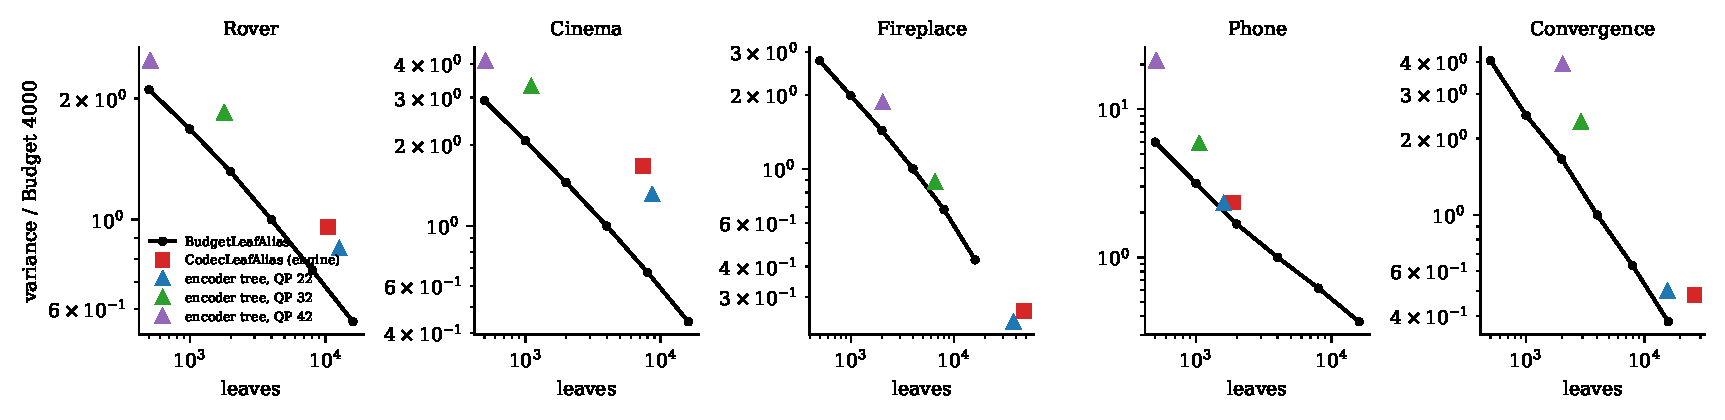
\includegraphics[width=\linewidth]{variance_vs_leaves.pdf}
\caption{Light-sampling variance against leaf count, relative to BudgetLeafAlias with 4000 leaves (median over frames). The black curve is BudgetLeafAlias from 500 to 16000 leaves; points are the codec partitions. A point above the curve reaches less quality than the budget tree with the same number of leaves.}
\label{fig:curve}
\end{figure}

\begin{table}[H]
\centering\small
\setlength{\tabcolsep}{4pt}
\begin{tabular}{llrrrr}
\toprule
Scene & Partition & Leaves (median, range) & Memory & $V$ / Budget 4000 & Leaf usefulness \\
\midrule
Rover & CodecLeafAlias (engine) & 10474 (8841--13257) & 495\,KB & 0.96 & 0.43 \\
 & Encoder tree, QP 32 & 1796 (1281--2331) & 190\,KB & 1.84 & 0.40 \\
Cinema & CodecLeafAlias (engine) & 7386 (3924--10029) & 386\,KB & 1.67 & 0.23 \\
 & Encoder tree, QP 32 & 1110 (606--2004) & 166\,KB & 3.30 & 0.41 \\
Fireplace & CodecLeafAlias (engine) & 47462 (44475--102516) & 2.2\,MB & 0.26 & 0.54 \\
 & Encoder tree, QP 32 & 6558 (6084--7026) & 737\,KB & 0.88 & 0.77 \\
Phone & CodecLeafAlias (engine) & 1872 (528--20133) & 192\,KB & 2.34 & 0.94 \\
 & Encoder tree, QP 32 & 1056 (510--4215) & 164\,KB & 5.84 & 0.86 \\
Convergence & CodecLeafAlias (engine) & 26696 (7287--38685) & 1.4\,MB & 0.48 & 0.40 \\
 & Encoder tree, QP 32 & 2906 (2559--3129) & 608\,KB & 2.32 & 0.42 \\
\midrule
All scenes & BudgetLeafAlias, $B=4000$ & 4000 (fixed) & 75\,KB & 1 & 1 \\
\bottomrule
\end{tabular}
\caption{Medians over the sampled frames. Leaf usefulness is the equivalent budget divided by the partition's own leaf count. Memory: 19 bytes per leaf for BudgetLeafAlias; 36 bytes per leaf plus a $W/8\times H/8$ leaf map for the codec partitions.}
\label{tab:main}
\end{table}

\begin{figure}[H]
\centering
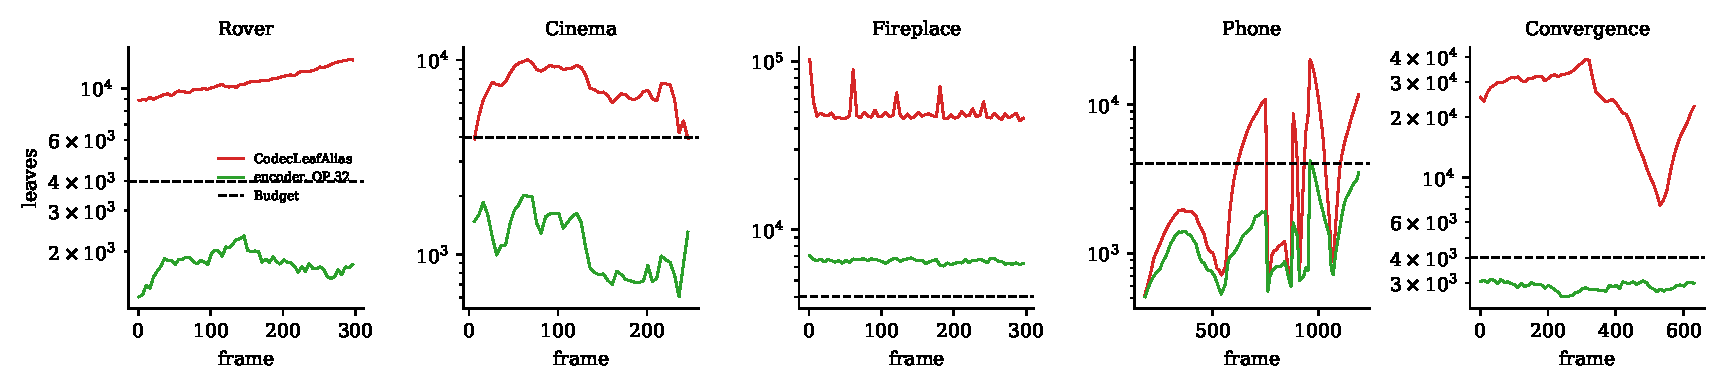
\includegraphics[width=\linewidth]{leaves_over_time.pdf}
\caption{Leaf count over each video: the engine's codec partition, the encoder tree at QP 32, and the fixed budget (dashed).}
\label{fig:time}
\end{figure}

\textbf{Codec leaves are placed less usefully.} In every scene the codec partitions lie above the budget curve (Figure~\ref{fig:curve}): BudgetLeafAlias reaches the same variance with 23--77\% of their leaves (Table~\ref{tab:main}; Phone, at 0.86--0.94, is the closest). The reason is what the partitions follow. A codec splits blocks where the picture has visible detail, measured on perceptually coded luma or as relative contrast, regardless of how much light the block emits. In Cinema, a dark film frame, 66\% of the engine partition's leaves together hold less than 1\% of the frame's light, against 15\% for the budget tree; the encoder tree at QP 32 puts 52\% of its leaves there.

\textbf{Where codec metadata helps.} When the partition comes with many more leaves than the budget, it can beat it in absolute terms. In Fireplace the engine partition has about 47000 leaves, 12 times the budget, and reaches 0.26 of its variance; in Convergence it has about 27000 and reaches 0.48. The same holds for an encoder at high quality (QP 22: 0.24 and 0.50). Rendered at equal samples, CodecLeafAlias is accordingly 5.3\% better than BudgetLeafAlias in Fireplace and 1.7\% better in Convergence, and at equal time it leads in Fireplace, Phone and Convergence. The partition costs the renderer nothing to compute when it is read from the stream, and a codec builds it in hardware.

\textbf{Where it fails.}
\begin{itemize}\setlength{\itemsep}{0pt}
\item \emph{At ordinary bitrates.} At QP 32 an encoder keeps 1000--6600 leaves, and its variance is 1.8 to 5.8 times that of the budget tree in four scenes; at QP 42 it falls to the minimum of one leaf per $64\times64$ block and the variance is 1.9 to 21 times higher. The quality of the light density then depends on a rate decision made for compression.
\item \emph{On dark or low-contrast content.} Cinema's engine partition has 7400 leaves and still 1.67 times the variance of 4000 budget leaves, because most of its leaves sit in dark detail.
\item \emph{When the leaf count swings.} Within one video the codec leaf count varies by 40 times in Phone (528 to 20133) and 5 times in Convergence (Figure~\ref{fig:time}), and in Phone's darkest frames the codec partition is hundreds of times worse than the budget (95th percentile of $V$ ratio: 300). Memory, cache footprint and sampling cost vary with it: 0.2 to 2.2\,MB per frame, against a fixed 75\,KB.
\end{itemize}

\textbf{When to use a budget.} BudgetLeafAlias gives the most light-sampling quality per leaf in every scene, a fixed memory footprint that stays in the GPU's first-level cache, and a sampling cost that does not depend on the content or the bitrate. It needs no codec, so it also applies to rendered, procedural or uncompressed emissive textures. Its limit is the budget itself: in scenes where light is concentrated in small regions, 4000 leaves leave some quality unused, and a budget of 8000--16000 recovers it at 2--4 times the memory (Fireplace: $V$ 0.42 at 16000 leaves).

\section*{3\quad When each is preferable}

\begin{itemize}\setlength{\itemsep}{0pt}
\item \textbf{CodecLeafAlias} when a decoded stream is at hand, the content is bright and detailed or the light is concentrated, the bitrate is high, and a variable memory footprint is acceptable: the partition is then free and has many leaves.
\item \textbf{BudgetLeafAlias} when memory or cache size must be bounded, at ordinary or low bitrates, on dark or fading content, for emissive textures that are not decoded from a stream, and whenever predictable cost matters.
\item A hybrid is natural: read the codec partition when it is available and cap or merge it to a budget of leaves by the same variance $\times$ area rule, which keeps the free partition's detail where the light is and bounds the memory.
\end{itemize}

\end{document}
